\documentclass[10pt,professionalfonts,serif,usenames,dvipsnames,svgnames,table]{beamer}

\usepackage{hyperref}
\hypersetup{
	pdfpagelabels=false
}

%\newenvironment{wideitemize}{\itemize\addtolength{\itemsep}{100pt}}{\enditemize}
%\newenvironment{wideenumerate}{\enumerate\addtolength{\itemsep}{100pt}}{\endenumerate}

%\usepackage{upquote}
%\usepackage{listings}
%\lstset{language=Python}
\usepackage{minted}

% turn off hyphenation
%\usepackage[none]{hyphenat}
%\usepackage{hyphenat}
%\raggedright

\usepackage{array}

\let\tempone\itemize
\let\temptwo\enditemize
\renewenvironment{itemize}{\tempone\addtolength{\itemsep}{0.5\baselineskip}}{\temptwo}

\let\tempthree\enumerate
\let\tempfour\endenumerate
\renewenvironment{enumerate}{\tempthree\addtolength{\itemsep}{0.5\baselineskip}}{\tempfour}

\usetheme{Singapore}

\definecolor{darkgreen}{rgb}{0, 0.5, 0.0}
\newcommand{\docutilsrolegreen}[1]{\color{darkgreen}#1\normalcolor}
\newcommand{\docutilsrolered}[1]{\color{red}#1\normalcolor}

\newcommand{\green}[1]{\color{darkgreen}#1\normalcolor}
\newcommand{\red}[1]{\color{red}#1\normalcolor}

\usepackage{lmodern}
%\usepackage{garamond}
\usepackage[garamond]{mathdesign}
%\usepackage[urw-garamond]{mathdesign}

%\usepackage{amsmath}
%\usepackage{amssymb}
%\usepackage{amsthm}
%\usepackage{amsfonts}
\usepackage{graphicx}
\usepackage{verbatim}
\usepackage{fancyvrb}
\usepackage{verbments}
\usepackage{colortbl}
\usepackage{slashed}
\usepackage{tabularx}
%\usepackage[normalem]{ulem}
\usepackage{multirow}
\usepackage{tikz}

\usepackage[loop, autoplay, buttonsize=1em, buttonbg=0, buttonfg=1]{animate}
\usepackage{movie15}

\providecommand\thispdfpagelabel[1]{}

\usetikzlibrary{shapes,arrows,trees}
\hypersetup{
colorlinks=true,
urlcolor=blue,
linkcolor=blue
}

%\usefonttheme[onlymath]{serif}
%\usecolortheme{orchid}
%\useinnertheme{rounded}

%\setbeamertemplate{headline}[default]
\setbeamercolor{author in head/foot}{fg=black,bg=white}
\setbeamercolor{title in head/foot}{fg=black,bg=white}
\setbeamercolor{date in head/foot}{fg=black,bg=white}

%\addtoheadtemplate{\pgfuseshading{beamer@headfade}\vskip-1.25cm}{}
%\usebackgroundtemplate{\includegraphics[width=\paperwidth,height=\paperheight]{images/bg.eps}}

%\setbeamercolor{frametitle}{bg=Blue,fg=white}
%\setbeamercolor{title}{bg=Blue,fg=white}

%\setbeamersize{text margin left=.2cm}
%\setbeamersize{text margin right=.5cm}

\setbeamertemplate{itemize itemsep}[0.3in]
\setbeamertemplate{itemize parsep}[0.3in]
\setbeamertemplate{enumerate itemsep}[0.3in]
\setbeamertemplate{enumerate parsep}[0.3in]

\setbeamertemplate{navigation symbols}{}
\setbeamersize{text margin left=.2cm,text margin right=.2cm}
\setbeamercovered{transparent}

\newcommand{\maxFrameImage}[1]
{
	{
	\setbeamercolor{background canvas}{bg=black,fg=white}
	\usebeamercolor[fg]{background canvas}
	\begin{frame}[plain]
	\begin{changemargin}{-1cm}{-1cm}
	\begin{center}
	\includegraphics[width=1.01\paperwidth,height=1.01\paperheight,keepaspectratio]{#1}
	\end{center}
	\end{changemargin}
	\end{frame}
	}
}

\newenvironment{changemargin}[2]{
	\begin{list}{}
	{
	\setlength{\topsep}{-3pt}
	\setlength{\leftmargin}{#1}
	\setlength{\rightmargin}{#2}
	\setlength{\listparindent}{\parindent}
	\setlength{\itemindent}{\parindent}
	\setlength{\parsep}{\parskip}
	}
	\item[]
}{\end{list}}

\newenvironment<>{varblock}[2][\textwidth]
{
	\setlength{\textwidth}{#1}
	\begin{actionenv}#3
	\def\insertblocktitle{#2}
	\par
	\usebeamertemplate{block begin}
	}
	{\pa
	\usebeamertemplate{block end}
	\end{actionenv}
}

\defbeamertemplate*{footline}{my theme}
{
  \leavevmode%
  \hbox{%
  \begin{beamercolorbox}[wd=.333333\paperwidth,ht=3.25ex,dp=1.25ex,left]{author in head/foot}%
    \usebeamerfont{author in head/foot}\hspace*{3.25ex}\insertshortauthor~~(\insertshortinstitute)
  \end{beamercolorbox}%
  \begin{beamercolorbox}[wd=.333333\paperwidth,ht=3.25ex,dp=1.25ex,center]{date in head/foot}%
    \usebeamerfont{date in head/foot}%\insertshortdate{}\hspace*{2em}
    {\large\insertframenumber{}}/\inserttotalframenumber{}
  \end{beamercolorbox}}%
  \begin{beamercolorbox}[wd=.333333\paperwidth,ht=3.25ex,dp=1.25ex,right]{title in head/foot}%
    \usebeamerfont{title in head/foot}\insertshorttitle\hspace*{3.25ex}
  \end{beamercolorbox}%
  \vskip0pt%
}


%
% SET UP DEFINITIONS IN HERE.  Make this one OFFICIAL MBC version!
%
%    11/14/00  copied from heprb. Last Update 10/20/00
%
%    6/25/97  all cplear stuff moved to cpleardef.tex
%
%     Latex stuff first:
%
% Set up better \caption command.  Both params are now mandatory
%\newcommand{\capt}[2]{ \begin{minipage}{0.8\textwidth} \caption[#1]{
%    \small #2} \end{minipage}  } 
%\newcommand{\capt}[3]{ \begin{minipage}{0.8\textwidth} \caption[#1]{
%    \small #2} \label{#3} \end{minipage}  } 
\newcommand{\ifm}[1]{\relax\ifmmode #1\else $#1$5\fi}
\newcommand{\capt}[3]{ \begin{minipage}{0.8\textwidth} \caption[#1]{
      \renewcommand{\baselinestretch}{1} \small #2} \label{#3} \end{minipage}  } 
\newcommand{\beq}{\begin{equation}}
\newcommand{\eeq}{\end{equation}}
\newcommand{\beqn}{\begin{eqnarray}}
\newcommand{\eeqn}{\end{eqnarray}}
\newcommand{\bi}{\begin{itemize}}
\newcommand{\ei}{\end{itemize}}
\newcommand{\bd}{\begin{description}}
\newcommand{\ed}{\end{description}}
\newcommand{\bHuge}{\begin{Huge}}
\newcommand{\bhuge}{\begin{huge}}
\newcommand{\bLARGE}{\begin{LARGE}}
\newcommand{\bLarge}{\begin{Large}}
\newcommand{\blarge}{\begin{large}}
\newcommand{\eHuge}{\end{Huge}}
\newcommand{\ehuge}{\end{huge}}
\newcommand{\eLARGE}{\end{LARGE}}
\newcommand{\eLarge}{\end{Large}}
\newcommand{\elarge}{\end{large}}
\def \mc {\multicolumn}
\def \mspace {\mbox{ }\mbox{ }\mbox{ }\mbox{ }}
%
\newcommand{\gt}{\ifm{>}}
\newcommand{\lt}{\ifm{<}}
\def \gtsim    {\relax\ifmmode{\mathrel{\mathpalette\oversim >}}
                  \else{$\mathrel{\mathpalette\oversim >}$}\fi}
\def \ltsim    {\relax\ifmmode{\mathrel{\mathpalette\oversim <}}
                  \else{$\mathrel{\mathpalette\oversim <}$}\fi}
\def\oversim#1#2{\lower4pt\vbox{\baselineskip0pt \lineskip1.5pt
            \ialign{$\mathsurround=0pt#1\hfil##\hfil$\crcr#2\crcr\sim\crcr}}}
\def \dk       {\relax\ifmmode{\rightarrow}\else{$\rightarrow$}4\fi}
\def \to       {\relax\ifmmode{\rightarrow}\else{$\rightarrow$}4\fi}
\def \Dk    {\relax\ifmmode{\Rightarrow}\else{$\Rightarrow$}\fi}
%\newcommand{\degr}{\mbox{$^{\circ}$}}
%
%
\newcounter{hours}\newcounter{minutes}
\newcommand{\printtime}{%
 	\setcounter{minutes}{\time}%
        \theminutes  min (since midnight)}
%
%
%
\newcommand{\vgap}{\vspace{0.5in}}
\newcommand{\hgap}{\hspace{0.5in}}
%
%
%%%%%   D0    %%%%%
%
\newcommand{\dzero}{\mbox{D\O}}
\newcommand{\Dzero}{\mbox{D\O}}
\newcommand{\DZERO}{\Dzero\ Collaboration}
%
%%%%%   CDF   %%%%%
%
\newcommand{\CDF}{CDF Collaboration}
\def \svx {SVX II}
\def \svxp {SVX$^{\prime}$}
%
%%%%% Event Topology %%%%%
%
\newcommand{ \Wjet}{\mbox{$W+{\rm jet}$}}
\newcommand{ \Njet}{\mbox{$N_{\rm jet}$}}

%%%%% HEP/Paricles %%%%%
%
%
%  standard model PARTICLES
%
\newcommand{ \lpm    }{\mbox{$\ell^{\pm}$}}
\newcommand{ \lmp    }{\mbox{$\ell^{\mp}$}}
\newcommand{ \lplm    }{\mbox{$\ell^{+} \ell^{-}$}}
\newcommand{ \epm    }{\mbox{$e^{\pm}$}}
\newcommand{ \eplus    }{\mbox{$e^{+}$}}
\newcommand{ \eminus    }{\mbox{$e^{-}$}}
\newcommand{ \lplus  }{\mbox{$\ell^+$}}
\newcommand{ \lminus }{\mbox{$\ell^-$}}
\newcommand{ \taul}{\mbox{$\tau_{\ell}$}}
\newcommand{ \tauh}{\mbox{$\tau_{\rm h}$}}
\newcommand{\ee}{\mbox{$ee$}}
\newcommand{\lnu}{\mbox{$\ell \nu$}}
\newcommand{\emu}{\mbox{$e\mu$}}
\newcommand{\mumu}{\mbox{$\mu\mu$}}
\newcommand{\epem}{\mbox{$e^+e^-$}}
\newcommand{\mpmm}{\mbox{$\mu^+\mu^-$}}
%
\newcommand{\qbar}   {\mbox{$\overline{q}$}}
\newcommand{\cbar}   {\mbox{$\overline{c}$}}
\newcommand{\bbar}   {\mbox{$\overline{b}$}}
\newcommand{\tbar}   {\mbox{$\overline{t}$}}
\newcommand{\ppbar}{\mbox{$p\overline{p}$}}
\newcommand{\ppb}{\mbox{$p\overline{p}$}}
\newcommand{\bbbar}{\mbox{$b\overline{b}$}}
\newcommand{\bbb}{\mbox{$b\overline{b}$}}
\newcommand{\ccbar}{\mbox{$c\overline{c}$}}
\newcommand{\ccb}{\mbox{$c\overline{c}$}}
\newcommand{\qqbar}{\mbox{$q\overline{q}$}}
\newcommand{\ttbar}{\mbox{$t\overline{t}$}}
\newcommand{\ttb}{\mbox{$t\overline{t}$}}
%
\newcommand{\wpm}{\mbox{$W^{\pm}$}}
\newcommand{\Wpm}{\mbox{$W^{\pm}$}}
\newcommand{\Wp}{\mbox{$W^{+}$}}
\newcommand{\Wm}{\mbox{$W^{-}$}}
\newcommand{\zzero}{\mbox{$Z^0$}}
\newcommand{\zz}{\mbox{$Z^0$}}
\newcommand{\Zz}{\mbox{$Z^0$}}
\newcommand{\wb}{\ifm{W}}
\newcommand{\zb}{\ifm{Z}}
%
\newcommand{\mets}{\mbox{${E\!\!\!\!/_{\rm T}}$}}
\newcommand{\met}{\mbox{${E\!\!\!\!/_{\rm T}}$}}
\newcommand{\metvec}{\mbox{${\vec{E}\!\!\!\!/_{\rm T}}$}}
%
\newcommand{\rp}{\mbox{${R_p}$}}
\newcommand{\rpc}{\mbox{${R_p}$}}
\newcommand{\rpv}{\mbox{${R\!\!\!\!\!\:/_p}$}}
\newcommand{\lnv}{\mbox{${L\!\!\!\!\!\:/}$}}
\newcommand{\bnv}{\mbox{${B\!\!\!\!\!\:/}$}}
\newcommand{\lamp}{\mbox{${\lambda^{\prime}_{121}}$}}
%
\newcommand{\lum}{\mbox{${\cal L}$}}
\newcommand{\br}{\mbox{${\cal B}$}}
\newcommand{\intlum}{\mbox{${ \int {\cal L} \; dt}$}}
\newcommand{\pt}{\mbox{$p_{{\rm T}}$}}
\newcommand{\pttauh}{\mbox{$p_{{\rm T}^{\tau_h} }$}}
\newcommand{\pT}{\mbox{$p_{{\rm T}}$}}
\newcommand{\Pt}{\mbox{$p_{{\rm T}}$}}
\newcommand{\ipt}{\mbox{$p^{-1}_{{\rm T}}$}}
\newcommand{\ptcut}{\mbox{$p_{{\rm T}}$-Cut}}
\newcommand{\et}{\mbox{$E_{{\rm T}}$}}
\newcommand{\Et}{\mbox{$E_{{\rm T}}$}}
\newcommand{\ET}{\mbox{$E_{{\rm T}}$}}
\newcommand{\sigpt}{\mbox{$\sigma_{\pT}/\pT$}}
\newcommand{\dphi}{\mbox{$\Delta\varphi$}}
\newcommand{\Ht}{\ifm{H_{{\rm T}}}}
\newcommand{\St}{\ifm{S_{{\rm T}}}}
\newcommand{\abseta}{\ifm{|\eta|}}
\newcommand{\Mt}{\mbox{$M_{{\rm T}}$}}
\newcommand{\mt}{\mbox{$m_{{\rm T}}$}}
%
%
%%%%% HEP/Ractions %%%%%
%
\newcommand{\Zee}{\mbox{$Z \rightarrow e^{+} e^{-}$}}
\newcommand{\Zmumu}{\mbox{$Z \rightarrow \mu^{+} \mu^{-}$}}
\newcommand{\Ztautau}{\mbox{$Z \rightarrow \tau^{+} \tau^{-}$}}
\newcommand{\Wlnu}{\mbox{$W \rightarrow \ell \nu$}}
\newcommand{\Wtaulnu}{\mbox{$W \rightarrow \tau \nu \rightarrow \ell \nu \nu$}}
%
%%%%  mSUGRA parameters %%%%%
%
\newcommand{\azero}{\ifm{A_0}}
\newcommand{\tanb}{\ifm{\tan\beta}}
\newcommand{\mzero}{\ifm{m_0}}
\newcommand{\mhalf}{\ifm{m_{1/2}}}
%
%%%%  SUSY  %%%%%
%
\newcommand{ \photino}{\mbox{$\tilde{\gamma}$}}
\newcommand{ \gravitino} {\mbox{$\tilde{G}$}}
\newcommand{ \gluino} {\mbox{$\tilde{g}$}}
\newcommand{ \squark} {\mbox{$\tilde{q}$}}
\newcommand{ \squarkb} {\mbox{$\bar{\tilde{q}}$}}
\newcommand{ \slepton} {\mbox{$\tilde{\ell}$}}
\newcommand{ \seleR} {\mbox{$\tilde{e}_{R}$}}
\newcommand{ \seleRpm} {\mbox{$\tilde{e}_{R}^{\pm}$}}
\newcommand{ \seleL} {\mbox{$\tilde{e}_{L}$}}
\newcommand{ \seleLpm} {\mbox{$\tilde{e}_{L}^{\pm}$}}
\newcommand{ \sele} {\mbox{$\tilde{e}$}}
\newcommand{ \selepm} {\mbox{$\tilde{e}^{\pm}$}}
\newcommand{ \selep} {\mbox{$\tilde{e}^{+}$}}
\newcommand{ \selem} {\mbox{$\tilde{e}^{-}$}}
\newcommand{ \smu} {\mbox{$\tilde{\mu}$}}
\newcommand{ \smuR} {\mbox{$\tilde{\mu}_R$}}
\newcommand{ \smuRpm} {\mbox{$\tilde{\mu}_R^{\pm}$}}
\newcommand{ \smupm} {\mbox{$\tilde{\mu}^{\pm}$}}
\newcommand{ \smup} {\mbox{$\tilde{\mu}^{+}$}}
\newcommand{ \smum} {\mbox{$\tilde{\mu}^{-}$}}
\newcommand{ \stauone} {\mbox{$\tilde{\tau}_{1}$}}
\newcommand{ \stauonep} {\mbox{$\tilde{\tau}_{1}^{+}$}}
\newcommand{ \stauonem} {\mbox{$\tilde{\tau}_{1}^{-}$}}
\newcommand{ \stauonepm} {\mbox{$\tilde{\tau}_{1}^{\pm}$}}
\newcommand{ \stau} {\mbox{$\tilde{\tau}$}}
\newcommand{ \stauL} {\mbox{$\tilde{\tau}_{L}$}}
\newcommand{ \stauR} {\mbox{$\tilde{\tau}_{R}$}}
\newcommand{ \staupm} {\mbox{$\tilde{\tau}^{\pm}$}}
\newcommand{ \staup} {\mbox{$\tilde{\tau}^{+}$}}
\newcommand{ \staum} {\mbox{$\tilde{\tau}^{-}$}}
\newcommand{ \snu}     {\mbox{$\tilde{\nu}$}}
\newcommand{ \sneutrino} {\mbox{$\tilde{\nu}$}}
\newcommand{ \usquark} {\mbox{$\tilde{u}$}}
\newcommand{ \dsquark} {\mbox{$\tilde{d}$}}
\newcommand{ \csquark} {\mbox{$\tilde{c}$}}
\newcommand{ \ssquark} {\mbox{$\tilde{s}$}}
\newcommand{ \scharm} {\mbox{$\tilde{c}$}}
\newcommand{ \csquarkl} {\mbox{$\tilde{c}_L$}}
\newcommand{ \csquarklb} {\mbox{$\bar{\tilde{c}}_L$}}
\newcommand{ \bcsquarkl} {\mbox{$\bar{\tilde{c}}_L$}}
\newcommand{ \bsquark} {\mbox{$\tilde{b}$}}
\newcommand{ \tsquark} {\mbox{$\tilde{t}$}}
\newcommand{ \sbottom}    {\mbox{$\tilde{b}$}}
\newcommand{ \sbottomb}    {\mbox{$\bar{\tilde{b}}$}}
\newcommand{ \sbottomone}    {\mbox{$\tilde{b}_{1}$}}
\newcommand{ \sbottomoneb}    {\mbox{$\bar{\tilde{b}}_{1}$}}
\newcommand{ \sstop}    {\mbox{$\tilde{t}$}}
\newcommand{ \stopo}   {\mbox{$\tilde{t}_{1}$}}
\newcommand{ \stopone}    {\mbox{$\tilde{t}_{1}$}}
\newcommand{ \stoponeb}    {\mbox{$\bar{\tilde{t}}_{1}$}}
\newcommand{ \stoptwo}    {\mbox{$\tilde{t}_{2}$}}
\newcommand{ \stopr}    {\mbox{$\tilde{t}_{R}$}}
\newcommand{ \stopl}    {\mbox{$\tilde{t}_{L}$}}
\newcommand{ \stoptwob}    {\mbox{$\bar{\tilde{t}}_{2}$}}
\newcommand{\sfermion}{\mbox{$\widetilde f$}}
%
\newcommand{ \cscsb}   {\mbox{$\csquarkl\bcsquarkl$}}
\newcommand{ \sqsq}   {\mbox{$\squark\squark$}}
\newcommand{ \sqsqb}   {\mbox{$\squark\squarkb$}}
\newcommand{ \ssb}     {\mbox{$\squark\overline{\squark}$}}
\newcommand{ \ststbone}   {\mbox{$\stopone\stoponeb$}}
\newcommand{ \ttbone}   {\mbox{$\stopone\stoponeb$}}
\newcommand{ \ttbtwo}   {\mbox{$\stoptwo\stoptwob$}}
%
\newcommand{ \cgino}{\mbox{$\tilde{\chi}^{\pm}$}}
\newcommand{ \nlino}{\mbox{$\tilde{\chi}^{0}$}}
\newcommand{ \ngino}{\mbox{$\tilde{\chi}^{0}$}}
\newcommand{ \wino}   {\mbox{$\tilde{W}^{\pm}$}}
\newcommand{ \zino}   {\mbox{$\tilde{Z}$}}
\newcommand{ \schi }{\mbox{$\tilde{\chi}$}}
\newcommand{ \lsp}    {\mbox{$\tilde{\chi}_{1}^{0}$}}
\newcommand{ \schionezero }{\mbox{$\tilde{\chi}_{1}^{0}$}}
\newcommand{ \schitwozero }{\mbox{$\tilde{\chi}_{2}^{0}$}}
\newcommand{ \schithreezero }{\mbox{$\tilde{\chi}_{3}^{0}$}}
\newcommand{ \schifourzero }{\mbox{$\tilde{\chi}_{4}^{0}$}}
\newcommand{ \schionepm }{\mbox{$\tilde{\chi}_{1}^{\pm}$}}
\newcommand{ \schionep }{\mbox{$\tilde{\chi}_{1}^{+}$}}
\newcommand{ \schionem }{\mbox{$\tilde{\chi}_{1}^{-}$}}
\newcommand{ \schitwopm }{\mbox{$\tilde{\chi}_{2}^{\pm}$}}
\newcommand{ \schitwop }{\mbox{$\tilde{\chi}_{2}^{+}$}}
\newcommand{ \schitwom }{\mbox{$\tilde{\chi}_{2}^{-}$}}
%
\newcommand{ \chizero}{\mbox{$\tilde{\chi}_{1}^0$}}
\newcommand{ \chione }{\mbox{$\tilde{\chi}_{1}^{\pm}$}}
\newcommand{ \chionemp }{\mbox{$\tilde{\chi}_{1}^{\mp}$}}
\newcommand{ \chipm  }{\mbox{$\tilde{\chi}^{\pm}$}}
\newcommand{ \chimp  }{\mbox{$\tilde{\chi}^{\mp}$}}
\newcommand{ \chip  }{\mbox{$\tilde{\chi}^{+}$}}
\newcommand{ \chim  }{\mbox{$\tilde{\chi}^{-}$}}
\newcommand{ \chionep   }{\mbox{$\tilde{\chi}_{1}^{+}$}}
\newcommand{ \chionem   }{\mbox{$\tilde{\chi}_{1}^{-}$}}
\newcommand{ \chitwo }{\mbox{$\tilde{\chi}_{2}^0$}}
\newcommand{ \chichi} {\mbox{$\chione\chitwo$}}
%
\newcommand{ \Mgluino} {\mbox{$M(\gluino)$}}
\newcommand{ \Msquark} {\mbox{$M(\squark)$}}
\newcommand{ \Mcsl} {\mbox{$M(\csquarkl)$}}
\newcommand{ \Msbotone} {\mbox{$M(\tilde{b}_{1})$}}
\newcommand{ \Mstopone} {\mbox{$M(\tilde{t}_{1})$}}
\newcommand{ \mstopo}   {\mbox{$m(\tilde{t}_1)$}}	% use lower case "m" (1/09/05)
\newcommand{ \Mchizero}{\mbox{$M(\chizero)$}}
\newcommand{ \Mchionepm}{\mbox{$M(\schionepm)$}}
\newcommand{ \sqmass }{\mbox{$M_{\tilde{q}}$}}
\newcommand{ \glmass }{\mbox{$M_{\tilde{g}}$}}
\newcommand{ \hmass  }{\mbox{$M_{{H}^{\pm}}$}}
%
%%%%%%  OTHER    %%%%%%%
%
\newcommand{\dagg}[1]{ #1 ^{\dagger}}
% Define modulus command to give
% two vertical bars.
% Must be used in math mode.
\newcommand{\modulus}[1]{\left| #1 \right|}
\newcommand{\paren}[1]{\left( #1 \right)}
\newcommand{\ave}[1]{\left\langle #1 \right\rangle}
\newcommand{\mods}[1]{\left| #1 \right|^2}
\newcommand{\bra}[1]{\langle #1 |}
\newcommand{\ket}[1]{| #1 \rangle}
\newcommand{\braket}[2]{\langle #1 | #2 \rangle}
\newcommand{\bracket}[3]{\langle #1 | #2 | #3 \rangle}
\newcommand{\sqbs}[1]{\left[ #1 \right] }
\newcommand{\rea}[1]{\mbox{$\,{\rm Re}\left( #1 \right)$}}
\newcommand{\ima}[1]{\mbox{$\,{\rm Im}\left( #1 \right)$}}
%
\def \sp       {\relax\ifmmode{\;}\else{$\;$}\fi}	% T.Kamon (June 1997)
%
%  Invariant masses, etc
%
\newcommand{\mll}{\mbox{$M(\ell\ell)$}}
\newcommand{\mjj}{\mbox{$M(jj)$}}
\newcommand{\mlljj}{\mbox{$M(\ell\ell jj)$}}
\newcommand{\dphill}{\mbox{$\Delta \phi (\ell\ell)$}}
\newcommand{\dphijj}{\mbox{$\Delta \phi (jj)$}}
%
%       Units
%
\newcommand{\mev}  {\mbox{${\rm MeV}/c$}}
\newcommand{\mevc} {\mbox{${\rm MeV}/c^2$}}
\newcommand{\gev}  {\mbox{${\rm GeV}$}}
\newcommand{\gevc} {\mbox{${\rm GeV}/c$}}
\newcommand{\pgev} {\mbox{${\rm GeV}/c$}}
\newcommand{\gevcc}{\mbox{${\rm GeV}/c^2$}}
\newcommand{\mmev}{\mbox{${\rm MeV}/c^2$}}
\newcommand{\mgev}{\mbox{${\rm GeV}/c^2$}}
\newcommand{\tev}  {\mbox{${\rm TeV}$}}
\newcommand{\mtev}{\mbox{${\rm TeV}/c^2$}}
\newcommand{\tevcc}{\mbox{${\rm TeV}/c^2$}}
\newcommand{\cmtwo}{\mbox{${\rm cm}^2$}}
%
%   luminosity
%
\newcommand{\invnb}{\mbox{${\rm nb}^{-1}$}}
\newcommand{\ipb}{\mbox{${\rm pb}^{-1}$}}
\newcommand{\invpb}{\mbox{${\rm pb}^{-1}$}}
\newcommand{\ifb}{\mbox{${\rm fb}^{-1}$}}
\newcommand{\invfb}{\mbox{${\rm fb}^{-1}$}}
\newcommand{\lumin}{\mbox{${\rm cm}^{-2}{\rm s}^{-1}$}}
%
%  Miscellaneous
%
\newcommand{\chis}{\mbox{$\chi^{2}$}}
\newcommand{\ie}{i.e.}
\newcommand{\eg}{e.g.}
\newcommand{\dedx}{\mbox{${\rm d}E/{\rm d}x$}}
\newcommand{\dndx}{\mbox{${\rm d}n/{\rm d}x$}}
\newcommand{\micron}{\mbox{$\mu{\rm m}$}}
\newcommand{\musec}{\mbox{$\mu {\rm s}$}}
\newcommand{\eps}{\mbox{$\epsilon$}}
\newcommand{\dxdy}{\mbox{${\rm d}X{\rm d}Y$}}
\newcommand{\sigrphi}{\mbox{$\sigma_{r \phi}$}}
\newcommand{\sigz}{\mbox{$\sigma_{z}$}}
\newcommand{\deltapp}{\mbox{$\Delta p/p$}} 
\newcommand{\degr}{\mbox{$^{\circ}$}} 

%
%-----------------------------------
% Publishing papers
%-----------------------------------
\def\Journal#1#2#3#4{{#1} {\bf #2}, #3 (#4)}
%
\def \PRL      {Phys. Rev. Lett.~}
\def \PR       {Phys. Rev.}
\def \PRD      {Phys. Rev. D}
\def \PL       {Phys. Lett.~}
\def \PLB      {Phys. Lett. B}
\def \ZPC      {Z. Phys. C}	% - Particles and Fields}
\def \NPB      {Nucl. Phys. B}
\def \PR       {Phys. Rep.~}
\def \INC      {Il Nuovo Cimento}
\def \NIM      {Nucl. Instrum. Methods}
\def \NIMA     {Nucl. Instrum. Methods Phys. Res. Sect. A}
\def \RPP	{Rep. Prog. Phys.}
\def \PRP	{Prog. Theor. Phys}
\def \MPL	{{Mod. Phys. Lett.} A}
\def \EPJC	{{Eur. Phys. J.} C}
\def \CPC	{Comput. Phys. Commun.}
%
%\def \etal     {\relax\ifmmode{et \; al. \;}\else{$et \; al. \;$}\fi}
\def \etal     {$et \; al. \;$}
%
%
%------------------------------------------------------------------------------
\newcommand{\GEANT}{{\sc geant}}
\newcommand{\PROSPINO}{{\sc prospino}}
\newcommand{\ISAJET}{{\sc isajet}}
\newcommand{\HERWIG}{{\sc herwig}}
\newcommand{\VECBOS}{{\sc vecbos}}
\newcommand{\PYTHIA}{{\sc pythia}}
%------------------------------------------------------------------------------


\title{rootpy: Pythonic ROOT}
%\subtitle{I have no subtitle}
\author[Noel Dawe]{Noel Dawe}
\date[\today]{\today}
\institute[rootpy]{for the rootpy dev team}
\titlegraphic{\includegraphics[height=3cm]{../common/images/rootpy_logo.png}}

\begin{document}

\frame{\titlepage}

\frame{
    \frametitle{What's the problem?}
    
    \begin{center}
    {\bf Why would we even consider developing a layer on top of PyROOT?}
    \end{center}

    \begin{itemize}
        \item PyROOT is mainly bindings with some pythonization.
        \item Certain tasks require awkward code. Same workarounds are
            implemented repetitively by many.
        \item Python's dynamic nature provides many possibilities although not
            currently realized by PyROOT.
        \item There is a lack of integration of ROOT with the vast and growing 
            ecosystem of scientific Python packages.
        \end{itemize}
}


\frame{
    \frametitle{Introducing rootpy}
    
    \begin{Large}
    \begin{center}
    \href{http://www.rootpy.org}{www.rootpy.org}
    \end{center}
    \end{Large}

    \begin{center}
    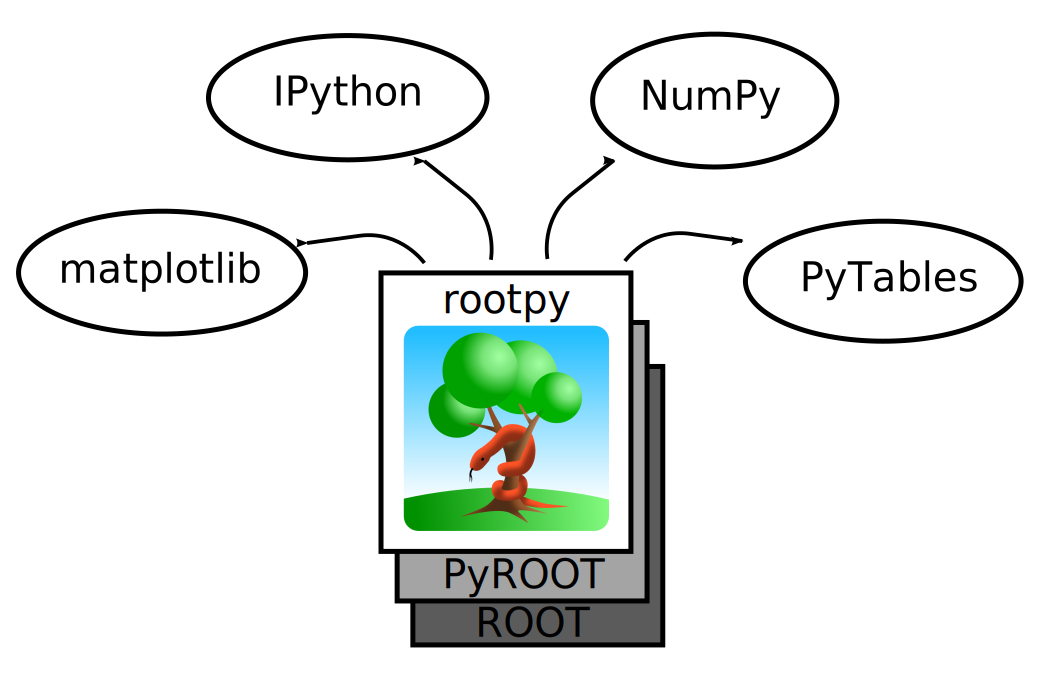
\includegraphics[height=.7\textheight]{figs/rootpy-map.png}
    \end{center}
}

\frame{
    \frametitle{rootpy: Design \& Philosophy}

    \begin{itemize}
        \item rootpy does not aim to reproduce ROOT in Python
        but rather provide a layer on top of PyROOT that integrates more
        naturally with Python:
        \vspace{.2cm}
        \begin{itemize}
            \itemsep=.2cm
            \item Setting and getting parameters with simple attributes:\\
                {\bf hist.linecolor = 'darkseagreen'}
            \item Simple navigation through TFiles:\\
                {\bf hist = myfile.somedirectory.otherdirectory.histname}
            \item Support for Python exceptions and logging
            \item Python has a garbage collector but C++ does not: leads to
                strange issues in PyROOT. rootpy addresses these problems.
            \item Arithmetic operators that are otherwise not implemented in
                PyROOT are implemented in rootpy
        \end{itemize}
    \end{itemize}
}

\frame{
    \frametitle{rootpy: Design \& Philosophy}

    \begin{itemize}
        \itemsep=.2cm
        \item rootpy classes simply inherit from the corresponding ROOT classes
            and may override methods to add functionality or be decorated with
            additional attributes
        \item rootpy classes typically have the same name as ROOT classes with
            the T removed
            but instead of having many histogram classes rootpy has three: Hist,
            Hist2D, Hist3D with a type argument in the constructor that controls
            which ROOT.THX is inherited from.
        \item Anywhere Python is typically slow (looping) is instead compiled as a C extension
            module. rootpy provides very fast conversion of ROOT Trees into
            NumPy arrays as well as efficiently filling ROOT histograms with
            NumPy arrays.

    \end{itemize}
}

\begin{frame}[fragile]
    \frametitle{rootpy example: opening a TFile}
    \begin{footnotesize}
\begin{minted}{python}

with get_file() as f:
    # access objects by name as properties of the current dir
    myhist = f.dimensions.hist2d
    # recursively walk through the file
    for path, dirs, objects in f.walk():
        print path, dirs, objects
\end{minted}
\end{footnotesize}

\end{frame}

\begin{frame}[fragile]
    \frametitle{rootpy example: creating histograms}
    \begin{Verbatim}[commandchars=\\\{\}]
\PY{k+kn}{from} \PY{n+nn}{rootpy.plotting} \PY{k+kn}{import} \PY{n}{Hist}\PY{p}{,} \PY{n}{Hist2D}\PY{p}{,} \PY{n}{Hist3D}

\PY{c}{\PYZsh{} create a 1D histogram}
\PY{n}{h} \PY{o}{=} \PY{n}{Hist}\PY{p}{(}\PY{l+m+mi}{10}\PY{p}{,} \PY{l+m+mi}{0}\PY{p}{,} \PY{l+m+mi}{1}\PY{p}{)}

\PY{c}{\PYZsh{} 2D and 3D histograms are handled in the same way}
\PY{c}{\PYZsh{} the constructor arguments are repetitions of \PYZsh{}bins, left bound, right bound.}
\PY{n}{h2d} \PY{o}{=} \PY{n}{Hist2D}\PY{p}{(}\PY{l+m+mi}{10}\PY{p}{,} \PY{l+m+mi}{0}\PY{p}{,} \PY{l+m+mi}{1}\PY{p}{,} \PY{l+m+mi}{50}\PY{p}{,} \PY{o}{-}\PY{l+m+mi}{40}\PY{p}{,} \PY{l+m+mi}{10}\PY{p}{,} \PY{n}{name}\PY{o}{=}\PY{l+s}{'}\PY{l+s}{2d hist}\PY{l+s}{'}\PY{p}{)}
\PY{n}{h3d} \PY{o}{=} \PY{n}{Hist3D}\PY{p}{(}\PY{l+m+mi}{3}\PY{p}{,} \PY{o}{-}\PY{l+m+mi}{1}\PY{p}{,} \PY{l+m+mi}{4}\PY{p}{,} \PY{l+m+mi}{10}\PY{p}{,} \PY{o}{-}\PY{l+m+mi}{1000}\PY{p}{,} \PY{o}{-}\PY{l+m+mi}{200}\PY{p}{,} \PY{l+m+mi}{2}\PY{p}{,} \PY{l+m+mi}{0}\PY{p}{,} \PY{l+m+mi}{1}\PY{p}{,} \PY{n}{name}\PY{o}{=}\PY{l+s}{'}\PY{l+s}{3d hist}\PY{l+s}{'}\PY{p}{)}

\PY{c}{\PYZsh{} variable-width bins may be created by passing the bin edges directly:}
\PY{n}{h1d\PYZus{}variable} \PY{o}{=} \PY{n}{Hist}\PY{p}{(}\PY{p}{[}\PY{l+m+mi}{1}\PY{p}{,} \PY{l+m+mi}{4}\PY{p}{,} \PY{l+m+mi}{10}\PY{p}{,} \PY{l+m+mi}{100}\PY{p}{]}\PY{p}{)}
\PY{n}{h2d\PYZus{}variable} \PY{o}{=} \PY{n}{Hist2D}\PY{p}{(}\PY{p}{[}\PY{l+m+mi}{2}\PY{p}{,} \PY{l+m+mi}{4}\PY{p}{,} \PY{l+m+mi}{7}\PY{p}{,} \PY{l+m+mi}{100}\PY{p}{,} \PY{l+m+mi}{200}\PY{p}{]}\PY{p}{,} \PY{p}{[}\PY{o}{-}\PY{l+m+mi}{100}\PY{p}{,} \PY{o}{-}\PY{l+m+mi}{50}\PY{p}{,} \PY{l+m+mi}{0}\PY{p}{,} \PY{l+m+mi}{10}\PY{p}{,} \PY{l+m+mi}{20}\PY{p}{]}\PY{p}{)}
\PY{n}{h3d\PYZus{}variable} \PY{o}{=} \PY{n}{Hist3D}\PY{p}{(}\PY{p}{[}\PY{l+m+mi}{1}\PY{p}{,} \PY{l+m+mi}{3}\PY{p}{,} \PY{l+m+mi}{10}\PY{p}{]}\PY{p}{,} \PY{p}{[}\PY{l+m+mi}{20}\PY{p}{,} \PY{l+m+mi}{50}\PY{p}{,} \PY{l+m+mi}{100}\PY{p}{]}\PY{p}{,} \PY{p}{[}\PY{o}{-}\PY{l+m+mi}{10}\PY{p}{,} \PY{o}{-}\PY{l+m+mi}{5}\PY{p}{,} \PY{l+m+mi}{10}\PY{p}{,} \PY{l+m+mi}{20}\PY{p}{]}\PY{p}{)}

\PY{c}{\PYZsh{} variable-width and constant-width bins can be mixed:}
\PY{n}{h2d\PYZus{}mixed} \PY{o}{=} \PY{n}{Hist2D}\PY{p}{(}\PY{p}{[}\PY{l+m+mi}{2}\PY{p}{,} \PY{l+m+mi}{10}\PY{p}{,} \PY{l+m+mi}{30}\PY{p}{]}\PY{p}{,} \PY{l+m+mi}{10}\PY{p}{,} \PY{l+m+mi}{1}\PY{p}{,} \PY{l+m+mi}{5}\PY{p}{)}

\PY{c}{\PYZsh{} easily set visual attributes}
\PY{n}{h}\PY{o}{.}\PY{n}{linecolor} \PY{o}{=} \PY{l+s}{'}\PY{l+s}{blue}\PY{l+s}{'}
\PY{n}{h}\PY{o}{.}\PY{n}{fillcolor} \PY{o}{=} \PY{l+s}{'}\PY{l+s}{green}\PY{l+s}{'}
\PY{n}{h}\PY{o}{.}\PY{n}{fillstyle} \PY{o}{=} \PY{l+s}{'}\PY{l+s}{/}\PY{l+s}{'}
\end{Verbatim}

\end{frame}

\begin{frame}[fragile]
    \frametitle{rootpy example: filling a TTree}
    \begin{footnotesize}
\begin{pyglist}[language=python,texcl=true,style=vs,bgcolor=Moccasin]
from rootpy.io import open
from rootpy.tree import Tree, TreeModel
from rootpy.types import FloatCol, IntCol
import random

class Model(TreeModel):
    x = FloatCol(default=-1.)
    y = FloatCol()
    i = IntCol()

f = open('test.root', 'recreate')
tree = Tree(name='test', model=Model)

for i in xrange(100):
    tree.x = random.gauss(4, 3)
    tree.y = random.gauss(2, 3)
    tree.i = i
    tree.fill()

tree.write()
f.close()
\end{pyglist}
\end{footnotesize}

\end{frame}

\frame{
    \frametitle{The future of rootpy}

    \begin{itemize}
        \item Larger documentation coverage. This is important!
        \item More code examples.
        \item Python 3 is becoming more mainstream -- support for this in rootpy
            will be required.
        \item Better integration with the IPython prompt: full tab completion
            and addition of helpful builtin commands like pylab.
        \item Automatic wrapping of ROOT methods by parsing method signatures:
            \begin{itemize}
                \item If a method expects a TColor, rootpy can accept any matplotlib/ROOT color
                      and convert it into a TColor before passing to the ROOT method.
                \item Reduce the amount of code in rootpy.
                \end{itemize}
       \item TMVA:
           \begin{itemize}
                \item Feed TMVA NumPy arrays instead of TTrees. 
                \end{itemize}
       \item RooFit and RooStats:
           \begin{itemize}
                \item Wrap RooArgSet as set() and RooArgList as list()...
                \item Create RooDataSets from NumPy arrays.
                \end{itemize}
   \end{itemize}
}

\frame{
    \frametitle{How can I contribute?}
    
    \begin{itemize}
        \item We use Git! Development is community-driven.
        \item Just fork rootpy into your own GitHub account and:
    
            \hspace{1cm} {\bf git clone git@github.com:[username]/rootpy.git}

              Then submit a pull request with your contribution.
        \item Contributions are reviewed by peers before merging into the main branch.
        \item All new code is automatically tested against our test suite using
            \href{https://travis-ci.org/}{Travis CI}
    \end{itemize}
}

\end{document}
